%----------------------------------------------------------------------------------------
%	CHƯƠNG 3: PHƯƠNG PHÁP NGHIÊN CỨU VÀ THIẾT KẾ HỆ THỐNG
%----------------------------------------------------------------------------------------

\chapter{KIẾN TRÚC VÀ THIẾT KẾ HỆ THỐNG} % Tên của chương
\label{Chapter3}

% =================================================================
%   MỤC 3.1
% =================================================================
\section{Pipeline tổng thể của dự án}
\begin{center}
	\nopagebreak
	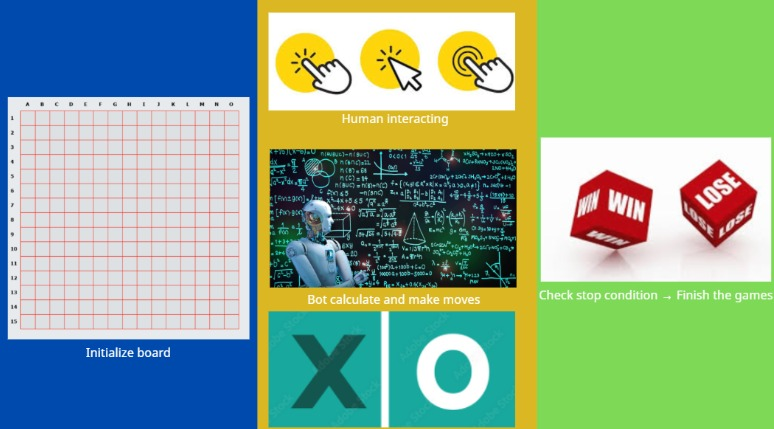
\includegraphics[width=\textwidth]{Figures/Gallery/pipeline.jpg}
	\captionof{figure}{Quy trình xử lý dữ liệu của hệ thống}
	\label{fig:pipeline}
\end{center}
\vspace{0.3cm}
Tiến trình xử lý và truyền dịch trạng thái của trò chơi được chia tách tường minh thành 4 giai đoạn cốt lõi bao gồm:

\begin{itemize}
	\item \textbf{Giai đoạn 1 - Khởi tạo cấu hình và Quản lý trạng thái gốc:} 
	Ngay khi ứng dụng được kích hoạt, hàm khởi tạo thiết lập các tham số kỹ thuật nền tảng bao gồm kích thước ma trận bàn cờ tiêu chuẩn ($10 \times 10$, $12 \times 12$, $15 \times 15$) và độ sâu cây quyết định mặc định cho AI ($\text{depth} = 3$). Hệ thống cấp phát vùng nhớ dọn trống toàn bộ ma trận về giá trị số $0$. Đặc biệt, cơ chế khóa bảo mật đồng bộ \texttt{threading.Lock()} được thiết lập sẵn nhằm chuẩn bị tài nguyên cho các tác vụ tính toán nền song song.
	
	\item \textbf{Giai đoạn 2 - Tương tác người dùng và Ghi nhận lịch sử di chuyển:} 
	Hệ thống lắng nghe các sự kiện phần cứng, đón nhận tọa độ click chuột $(r, c)$ từ người chơi (nhận giá trị toán học là $-1$). Hàm kiểm tra tính hợp lệ sẽ xác minh ô cờ trống trước khi ghi đè dữ liệu lên ma trận \texttt{board[r][c]}. Nước đi hợp lệ ngay lập tức được đóng gói dạng Tuple $(r, c, \text{player})$ đẩy vào ngăn xếp \texttt{move\_history}, đồng thời dịch mã sang định dạng biên bản cờ chuẩn hóa PGN để lưu vào \texttt{pgn\_history} trước khi chuyển đổi trạng thái lượt đi sang đối thủ.
	
	\item \textbf{Giai đoạn 3 - Giới hạn không gian và Tìm kiếm quyết định tối ưu (AI Decision Pipeline):} 
	Khi đến lượt đi của Bot AI (nhận giá trị toán học là $1$), hệ thống kích hoạt một luồng ngầm độc lập (\textit{Worker Thread}) để tránh gây nghẽn giao diện. Luồng phụ thực thi chuỗi tiến trình con:
	\begin{itemize}
		\item \textbf{Bước 1:} Gọi hàm \texttt{get\_interesting\_moves} quét ma trận trong bán kính 1 ô kế cận các quân cờ hiện hành để cô lập vùng tìm kiếm, giảm số lượng nút tiềm năng từ 150 ô xuống tối đa 30 ô để chặn đứng nguy cơ bùng nổ tổ hợp.
		\item \textbf{Bước 2:} Khởi chạy lõi Minimax đệ quy theo chiều sâu (DFS) xuống các tầng trạng thái giả lập.
		\item \textbf{Bước 3:} Xuyên suốt quá trình duyệt, hệ thống liên tục truyền các tham số chặn dưới $\alpha$ và chặn trên $\beta$, thực hiện bẻ gãy vòng lặp duyệt nhánh ngay khi phát hiện điều kiện $\alpha \ge \beta$.
		\item \textbf{Bước 4:} Tại độ sâu giới hạn, hàm \texttt{evaluate\_board\_heuristic} thực hiện cắt chuỗi con đối chiếu với từ điển \texttt{SCORE\_MATRIX} (kết hợp \texttt{ATTACK\_MATRIX} và \texttt{DEFEND\_MATRIX}) để tính toán điểm số tối ưu, trả về tọa độ nước đi tốt nhất tại nút gốc.
	\end{itemize}
	
	\item \textbf{Giai đoạn 4-- Xác định điều kiện dừng ván đấu (Terminal Check):} 
	Sau khi một nước đi được hạ xuống, hàm logic \texttt{check\_win} thực hiện nhiệm vụ quét trạng thái bàn cờ theo 4 hướng địa lý (ngang, dọc, và 2 đường chéo). Thuật toán áp dụng nghiêm ngặt luật chặn hai đầu tiêu chuẩn (\textit{Double-Blocked Rule}), tính toán biến \texttt{blocked\_ends} để đảm bảo chuỗi đạt $\ge 5$ quân cờ và không bị chặn cả 2 đầu thì mới phân định chiến thắng. Khi điều kiện dừng thỏa mãn (thắng-thua hoặc lấp đầy bàn cờ dẫn đến hòa), trạng thái \texttt{game\_over} được gán bằng \texttt{True} để đóng băng tương ứng, đồng thời kích hoạt hàm \texttt{print\_pgn\_final()} xuất toàn bộ biên bản trận đấu ra màn hình điều khiển.
\end{itemize}

\section{Chi tiết kiến trúc phần mềm và cài đặt thuật toán}
\subsection{Thiết kế Module}

Một trong những điểm cải tiến cốt lõi trong kiến trúc phần mềm của đề tài này là việc áp dụng nguyên lý phân tách các thành phần. Thay vì xây dựng một tệp mã nguồn tập trung, hệ thống được chia thành hai module độc lập, giao tiếp với nhau thông qua lập trình hướng đối tượng:
\begin{itemize}
	\item \textbf{Module bộ não xử lý trung tâm (Logic\_game.py):} Đây là thành phần chứa toàn bộ trạng thái dữ liệu của ván cờ. Lớp này chịu trách nhiệm khởi tạo ma trận bàn cờ, ghi nhận lịch sử nước đi, kiểm tra điều kiện chiến thắng và thực thi các giải thuật Minimax, Heuristic. Điểm đặc biệt là lớp CaroLogic hoàn toàn độc lập với môi trường đồ họa, không chứa bất kỳ mã nguồn nào liên quan đến thư viện hiển thị Pygame, giúp nó có tính tái sử dụng cao.
	\item \textbf{Module giao diện đồ họa (UI.py):} Thành phần này đóng vai trò là giao diện tương tác trực tiếp với người sử dụng. Nó chịu trách nhiệm khởi tạo cửa sổ ứng dụng bằng thư viện Pygame, hiển thị hình ảnh màu sắc hệ Dark Mode, quản lý hệ thống âm thanh hiệu ứng (SFX) và lắng nghe các sự kiện phần cứng như click chuột hoặc nhập liệu văn bản.
\end{itemize}

\subsection{Quản lý trạng thái và tính năng bổ trợ (State Management)}
Trạng thái của một ván cờ được lớp \texttt{CaroLogic} quản lý động thông qua hệ thống lưu vết lịch sử di chuyển, cho phép triển khai các tính năng bổ trợ nâng cao nhằm tối ưu hóa trải nghiệm người dùng:
\begin{itemize}
	\item \textbf{Cơ chế hoạt động của tính năng Undo (Đi lại):} Tính năng này được cài đặt dựa trên cấu trúc dữ liệu Ngăn xếp (\textit{Stack}) tuyến tính. Toàn bộ các nước đi của người chơi và Bot AI sau khi thực hiện thành công sẽ được đóng gói dưới dạng Tuple $(r, c, \text{player})$ và đẩy vào mảng \texttt{move\_history}. Đồng thời, ký hiệu định dạng biên bản PGN cũng được lưu vào \texttt{pgn\_history}. Khi người chơi kích hoạt lệnh Undo (thông qua phím tắt U trên bàn phím hoặc click nút UNDO trên Control Panel), hàm \texttt{undo\_move} sẽ thực hiện lệnh giải phóng bộ nhớ bằng cách rút (\texttt{.pop()}) liên tiếp hai phần tử cuối cùng ra khỏi ngăn xếp lịch sử (tương ứng với một nước cờ của máy và một nước cờ của người). Hệ thống tiến hành đặt lại giá trị ma trận tại hai vị trí đó về bằng $0$ (ô trống), xóa biên bản tương ứng và trả lại lượt đi cho con người.
	\item \textbf{Cơ chế hoạt động của tính năng Reset (Làm mới) và Menu Trận đấu:} Tính năng Reset (phím tắt R hoặc nút RESET) kích hoạt hàm \texttt{reset\_game} giúp xóa trắng toàn bộ ma trận bàn cờ về $0$ và dọn rác các mảng lịch sử mà không cần phải khởi động lại toàn bộ chương trình. Trong khi đó, vòng lặp \texttt{show\_menu} cung cấp một giao diện cấu hình trực quan trước trận đấu. Người dùng có thể tác động lên các nút bấm để thay đổi trực tiếp các tham số cấu hình của lớp \texttt{CaroLogic} bao gồm kích thước ma trận (\texttt{board\_size} nhận các giá trị $10, 12, 15$) và độ sâu cây tìm kiếm quyết định (\texttt{bot\_depth} nhận các giá trị $1, 2, 3$).
\end{itemize}

\subsection{Tối ưu hóa hiệu năng bằng Đa luồng (Multi-threading)}
Đối với các ứng dụng giao diện đồ họa (GUI), việc duy trì tốc độ phản hồi mượt mà của khung hình là yếu tố tiên quyết. Tuy nhiên, thuật toán tìm kiếm Minimax ở độ sâu lớn ($\text{Depth} = 3$) đòi hỏi một khối lượng tính toán khổng lồ và tốn từ 1 đến vài giây để đưa ra kết quả. Nếu tiến trình này được thực thi trực tiếp trên luồng chạy chính (\textit{Main Thread} - nơi đảm nhận nhiệm vụ vẽ giao diện và bắt sự kiện Pygame), hệ điều hành sẽ rơi vào trạng thái tắc nghẽn, gây ra hiện tượng treo cửa sổ.

Để giải quyết triệt để bài toán hiệu năng này, hệ thống áp dụng kỹ thuật Lập trình đa luồng (\textit{Multi-threading}) thông qua thư viện \texttt{threading} tích hợp sẵn của Python:
\begin{itemize}
	\item \textbf{Phân chia luồng xử lý (Threading Workers):} Luồng chính (\textit{Main Thread}) được giải phóng hoàn toàn khỏi các tác vụ tính toán nặng, chỉ tập trung duy nhất vào vòng lặp vẽ màn hình \texttt{draw\_ui} cố định ở tốc độ $30$ khung hình/giây ($30$ FPS). Khi đến lượt của Bot AI di chuyển hoặc khi người chơi nhấn nút yêu cầu trợ giúp nước đi, lớp \texttt{CaroUI} sẽ lập tức khởi tạo một luồng ngầm độc lập (\textit{Worker Thread}) thông qua lệnh \texttt{threading.Thread(target=..., daemon=True).start()} tương ứng cho các hàm \texttt{bot\_calculation\_worker} hoặc \texttt{hint\_calculation\_worker}. Tiến trình tính toán Minimax sẽ chạy song song ở chế độ nền. Khi tìm ra nước đi tối ưu, luồng phụ này sẽ cập nhật kết quả vào bộ nhớ chung và tự động kết thúc ván đóng luồng.
	\item \textbf{Cơ chế Khóa bảo mật đồng bộ (\texttt{threading.Lock}):} Do hệ thống vận hành theo mô hình đa luồng truy cập đồng thời vào một vùng tài nguyên chung (Ma trận dữ liệu \texttt{self.logic.board}), nguy cơ xảy ra lỗi tranh chấp dữ liệu (\textit{Race Condition}) là cực kỳ cao. Ví dụ: luồng chính đang đọc ma trận để vẽ quân cờ lên màn hình trong khi luồng phụ AI đang ghi đè thay đổi giá trị để giả lập nước đi Minimax. Để ngăn chặn xung đột, nhóm sử dụng cơ chế khóa đồng bộ độc quyền thông qua đối tượng \texttt{self.lock = threading.Lock()} trong lớp \texttt{CaroLogic}. Bằng cú pháp \texttt{with self.logic.lock:} (hoặc \texttt{with self.lock:}), luồng đang thực thi sẽ chiếm quyền kiểm soát két sắt dữ liệu, ép tất cả các luồng khác phải rơi vào trạng thái chờ (\textit{Block}) cho đến khi luồng hiện tại xử lý xong dòng code và mở khóa. Cơ chế này đảm bảo tính toàn vẹn dữ liệu tuyệt đối cho hệ thống trò chơi.
\end{itemize}

\subsection{Cài đặt thuật toán hệ thống}

\subsubsection{Thiết lập trọng số Hàm đánh giá}
Trọng tâm sức mạnh tư duy của Bot AI nằm ở việc thiết lập các giá trị hằng số trong bộ từ điển điểm số \texttt{SCORE\_MATRIX}. Để tạo ra một đối thủ có lối chơi thực tế, thông minh và biết tùy biến theo thế trận, nhóm đã áp dụng chiến lược lai giữa cấu trúc mẫu hình hình học (\textit{Pattern Matching}) và tư duy công -- thủ biệt lập:
\begin{itemize}
	\item \textbf{Chiến lược ma trận tấn công (\texttt{ATTACK\_MATRIX}):} Định nghĩa giá trị điểm số dương cho các chuỗi quân cờ của riêng AI (mang giá trị $1$ trên ma trận). Điểm số được phân cấp nhảy vọt để ưu tiên tuyệt đối cho các nước đi dứt điểm ván đấu: chuỗi 5 quân thắng chắc nhận $200.000$ điểm, thế cờ 4 quân mở 2 đầu nhận $11.000$ điểm, và giảm dần về các thế cờ tạo chuỗi 3 hoặc chuỗi 2.
	\item \textbf{Chiến lược ma trận phòng thủ (\texttt{DEFEND\_MATRIX}):} Định nghĩa giá trị điểm phạt (mang dấu âm) cho các cấu hình quân cờ của người chơi (mang giá trị $-1$ trên ma trận). 
	\item \textbf{Nguyên lý ép phòng thủ:} Điểm nhấn kỹ thuật đặc biệt ở đây là trị tuyệt đối của điểm phòng thủ luôn cao hơn điểm tấn công tại các ngưỡng thế cờ nguy cấp. Cụ thể, khi người chơi đạt thế 4 quân mở hai đầu, AI sẽ gán điểm phạt cực nặng là $-45.000$ điểm. Khi so sánh với điểm thưởng của thế tấn công 4 quân mở hai đầu của riêng mình ($11.000$ điểm), thuật toán Minimax buộc phải lựa chọn nước đi chặn đứng chuỗi cờ của đối thủ. Chiến lược này giúp AI ngăn chặn tối đa việc bị mắc bẫy ở các nước đi xa.
\end{itemize}

Sau khi định nghĩa, hai ma trận được gộp lại làm một thông qua cú pháp giải nén từ điển \texttt{SCORE\_MATRIX = \{**ATTACK\_MATRIX, **DEFEND\_MATRIX\}} của ngôn ngữ Python để thuật toán tìm kiếm tối ưu hóa tốc độ tra cứu cấu trúc dữ liệu với độ phức tạp $\mathcal{O}(1)$.

\begin{table}[!htbp]
	\centering
	\renewcommand{\arraystretch}{1.25}
	\caption{Bảng trọng số lượng giá trong cấu hình hàm đánh giá Heuristic}
	\label{tab:score_matrix}
	\begin{tabular}{|c|c|c|c|}
		\hline
		\textbf{Thế cờ (Pattern)} & \textbf{Trạng thái mô tả} & \textbf{Điểm Tấn công} & \textbf{Điểm Phòng thủ} \\ \hline
		\texttt{X X X X X} & 5 quân liên tiếp (Thắng) & $+200.000$ & $-200.000$ \\ \hline
		\texttt{- X X X X -} & 4 quân mở 2 đầu & $+11.000$ & $-45.000$ \\ \hline
		\texttt{O X X X X -} & 4 quân bị chặn 1 đầu & $+2.700$ & $-2.700$ \\ \hline
		\texttt{- X X X -} & 3 quân mở 2 đầu & $+670$ & $-1.500$ \\ \hline
		\texttt{- X X - X -} & 3 quân đứt đoạn & $+500$ & $-1.000$ \\ \hline
		\texttt{O X X X -} & 3 quân mở 1 đầu / Bị chặn & $+210$ & $-210$ \\ \hline
		\texttt{- X X -} & 2 quân mở 2 đầu & $+16$ & $-16$ \\ \hline
	\end{tabular}
\end{table}

\subsubsection{Cơ chế phân cấp 3 mức độ khó (\texttt{BOT\_DEPTH})}
Để trò chơi tiếp cận được nhiều đối tượng người dùng, lớp \texttt{CaroLogic} cài đặt biến cấu hình \texttt{bot\_depth} nhận 3 giá trị tương ứng với 3 cấp độ thông minh độc lập của Bot AI:
\begin{itemize}
	\item \textbf{Cấp độ Dễ (\texttt{bot\_depth} = 1):} Tại cấp độ này, thuật toán Minimax chỉ tìm kiếm ở độ sâu duy nhất là 1 bước đi kế tiếp. Đồng thời, tại hàm lọc nước đi, AI bị giới hạn nghiêm ngặt chỉ lấy 5 nước đi ngẫu nhiên đầu tiên xuất hiện trên bảng. Kết quả là AI chỉ có khả năng nhìn thấy các cơ hội ăn điểm trực tiếp hoặc nguy cơ thua ngay lập tức ở lượt sau, tạo nên một lối đánh ngây ngô, dễ mắc bẫy, phù hợp cho người chơi mới.
	\item \textbf{Cấp độ Trung bình (\texttt{bot\_depth} = 2):} Cây quyết định duyệt sâu xuống 2 tầng trạng thái (AI giả định nước đi của mình và một nước đáp trả tiếp theo của con người). Hàm lọc được nới rộng, tiến hành sắp xếp các nước đi tiềm năng theo bán kính tính từ tâm bàn cờ ra ngoài và cắt lấy tối đa 30 nước đi có điểm Heuristic cao nhất để đưa vào Minimax. Bot AI ở cấp độ này thời gian phản hồi rất nhanh, có khả năng phòng thủ và tấn công tương đối tốt nhưng thi thoảng vẫn bị lọt bẫy nếu người chơi kéo giãn quân cờ ra các vùng biên của bàn cờ.
	\item \textbf{Cấp độ Khó (\texttt{bot\_depth} = 3):} Thuật toán duyệt sâu xuống 3 tầng trạng thái đầy đủ trên cây quyết định. Ở cấp độ này, tham số giới hạn số lượng nước đi bị loại bỏ hoàn toàn, ép AI phải vét cạn tất cả các ô trống có khả năng phát sinh điểm. Kết hợp với việc cộng trừ tham số \texttt{depth} trực tiếp vào điểm số trả về ($1.000.000 + \text{depth}$ khi thắng hoặc $-1.000.000 - \text{depth}$ khi thua), AI được tối ưu hóa tư duy để luôn tìm cách chiến thắng với số nước đi ngắn nhất hoặc kéo dài sự sống lâu nhất có thể khi rơi vào thế thua.
\end{itemize}

\subsubsection{Thuật toán thu hẹp vùng tìm kiếm (\texttt{get\_interesting\_moves})}
Đối với một bàn cờ kích thước lớn như $15 \times 15$, tổng số ô trống ở giai đoạn giữa trận đấu có thể lên đến hơn $150$ ô. Nếu tung toàn bộ các ô trống này vào hàm đệ quy Minimax với $\text{Depth} = 3$, số lượng nút lá phát sinh trên cây quyết định sẽ tăng theo cấp số nhân ($150^3 = 3.375.000$ trạng thái), gây sập nguồn tài nguyên xử lý của CPU.

Để tối ưu hóa, nhóm đã cài đặt thuật toán lọc phân vùng thông minh thông qua hàm \texttt{get\_interesting\_moves}:
\begin{enumerate}
	\item Hàm tiến hành duyệt qua toàn bộ ma trận bàn cờ hiện tại.
	\item Tại các vị trí ô cờ đã được đánh quân, hàm sẽ quét rộng ra xung quanh theo 8 hướng hình học với bán kính rộng 1 ô cờ.
	\item Nếu phát hiện ô xung quanh là ô trống, tọa độ của ô đó sẽ được thêm vào cấu trúc dữ liệu \texttt{set()} (Tập hợp) nhằm tự động loại bỏ các tọa độ trùng lặp.
	\item Cuối cùng, tập hợp được chuyển đổi ngược về dạng mảng tuyến tính \texttt{move\_list}.
\end{enumerate}
Việc thu hẹp vùng tìm kiếm xuống bán kính 1 ô giúp AI cô lập hoàn toàn các ô trống vô ích ở vùng biên xa, giảm số lượng nước đi tiềm năng đưa vào Minimax từ $150$ ô xuống chỉ còn từ $15$ đến $35$ ô tùy giai đoạn trận đấu. Kỹ thuật này giúp giảm tải hơn $80\%$ khối lượng duyệt cây, đảm bảo thời gian tính toán nước đi chế độ Khó luôn duy trì ổn định.

\subsection{Ứng dụng mô hình Hồi quy Logistic trong tối ưu hóa bộ trọng số lượng giá}

Để loại bỏ tính cảm tính và tối ưu hóa các giá trị điểm số trong từ điển \texttt{SCORE\_MATRIX}, hệ thống triển khai mô hình học máy Hồi quy Logistic nhằm tự động hóa tiến trình khai phá dữ liệu và gán trọng số cho các mẫu hình chiến thuật. Quy trình hiện thực hóa giải pháp này được cấu trúc qua các giai đoạn tính toán chi tiết sau:

\subsubsection{Thu thập dữ liệu và biểu diễn không gian vectơ đặc trưng}
Dữ liệu huấn luyện được tổng hợp từ tập mẫu gồm các biên bản trận đấu chất lượng cao. Tại mỗi trạng thái bàn cờ $s$, cục diện được trích xuất và ánh xạ thành một vectơ đặc trưng $X = [x_1, x_2, \dots, x_n]^T$, trong đó mỗi phần tử $x_i$ đại diện cho tần suất xuất hiện $f_i(s)$ của mẫu hình thứ $i$ (ví dụ: số lượng thế cờ $4$ quân mở hai đầu, $3$ quân bị chặn một đầu).

Mỗi vectơ đặc trưng $X$ đi kèm với một nhãn mục tiêu nhị phân $y \in \{0, 1\}$ được xác định dựa trên kết quả cuối cùng của ván đấu:
\begin{equation}
	y = \begin{cases} 
		1 & \text{nếu trạng thái } s \text{ dẫn đến chiến thắng chung cuộc cho AI} \\
		0 & \text{nếu trạng thái } s \text{ dẫn đến thất bại hoặc hòa}
	\end{cases}
\end{equation}

\subsubsection{Cơ chế ước lượng xác suất bằng hàm kích hoạt phi tuyến}
Mô hình tiến hành thiết lập một hàm tổ hợp tuyến tính giữa vectơ đặc trưng $X$ và bộ trọng số hệ số hồi quy tương ứng $W = [w_1, w_2, \dots, w_n]^T$, kết hợp với sai số ngẫu nhiên $w_0$:
\begin{equation}
	z = w_0 + \sum_{i=1}^{n} w_i x_i
\end{equation}

Để chuyển đổi giá trị lượng giá $z$ từ không gian số thực vô hạn $(-\infty, +\infty)$ về không gian xác suất giới hạn $(0, 1)$, hệ thống đưa $z$ qua hàm kích hoạt Sigmoid toán học:
\begin{equation}
	P(y=1|X) = \hat{y} = \sigma(z) = \frac{1}{1 + e^{-z}}
\end{equation}
Trong đó, giá trị $\hat{y}$ phản ánh một cách chính xác tỷ lệ phần trăm cơ hội giành chiến thắng của tác tử AI khi sở hữu tổ hợp thế cờ hiện tại.

\subsubsection{Tối ưu hóa hàm mất mát và trích xuất điểm số Heuristic}
Quá trình huấn luyện mô hình thực chất là việc tìm kiếm bộ tham số $W$ sao cho khoảng cách giữa xác suất dự đoán $\hat{y}$ và nhãn thực tế $y$ là nhỏ nhất. Hệ thống áp dụng hàm mất mát Entropy chéo nhị phân (\textit{Binary Cross-Entropy Loss}) trên toàn bộ tập dữ liệu gồm $M$ mẫu:
\begin{equation}
	J(W) = -\frac{1}{M} \sum_{j=1}^{M} \left[ y^{(j)} \log(\hat{y}^{(j)}) + (1 - y^{(j)}) \log(1 - \hat{y}^{(j)}) \right]
\end{equation}

Thuật toán tối ưu hóa hạ gradient (\textit{Gradient Descent}) được kích hoạt để liên tục cập nhật trọng số theo chiều ngược pha với đạo hàm riêng:
\begin{equation}
	w_i \leftarrow w_i - \alpha \frac{\partial J(W)}{\partial w_i}
\end{equation}

Sau khi mô hình đạt trạng thái hội tụ, các hệ số hồi quy $w_i$ trích xuất được phản ánh trực tiếp mức độ đóng góp khoa học và tỷ lệ ảnh hưởng của từng mẫu hình đến khả năng chiến thắng cục diện. Khác với việc gán tay cảm tính, các hệ số thực nghiệm này tồn tại dưới dạng số thập phân có độ mịn cao. Hệ thống tiến hành chuẩn hóa và nạp trực tiếp các giá trị này vào hai ma trận \texttt{ATTACK\_MATRIX\_LOGISTIC} và \texttt{DEFEND\_MATRIX\_LOGISTIC} phục vụ cho lõi tìm kiếm Minimax, chi tiết thông số được thể hiện tại Bảng \ref{tab:weights_logistic}.

\begin{table}[!htbp]
	\centering
	\renewcommand{\arraystretch}{1.25}
	\caption{Hệ thống trọng số thực nghiệm tối ưu bằng Hồi quy Logistic}
	\label{tab:weights_logistic}
	\begin{tabular}{|c|c|c|c|}
		\hline
		\textbf{Thế cờ (Pattern)} & \textbf{Trạng thái mô tả} & \textbf{Điểm Tấn công} & \textbf{Điểm Phòng thủ} \\ \hline
		\texttt{X X X X X} & 5 quân liên tiếp (Thắng) & $+200.000,00$ & $-200.000,00$ \\ \hline
		\texttt{- X X X X -} & 4 quân mở 2 đầu & $+14.780,71$ & $-200.000,00$ \\ \hline
		\texttt{O X X X X -} & 4 quân bị chặn 1 đầu & $+18.888,35$ & $-23.248,95$ \\ \hline
		\texttt{- X X - X -} & 3 quân đứt đoạn & $+14.685,24$ & $-17.230,00$ \\ \hline
		\texttt{- X X X -} & 3 quân mở 2 đầu & $+2.908,00$ & $-3.550,76$ \\ \hline
		\texttt{O X X X -} & 3 quân mở 1 đầu & $+4.031,00$ & $-8.598,42$ \\ \hline
		\texttt{- X X -} & 2 quân mở 2 đầu & $+3.736,00$ & $-2.389,63$ \\ \hline
	\end{tabular}
\end{table}
Từ kết quả trên, ta có thể thấy thuật toán học máy đã tinh chỉnh bộ điểm số lệch hẳn so với việc gán tay cảm tính. Ví dụ, trạng thái phòng thủ chống lại chuỗi 4 quân mở 2 đầu (\texttt{- X X X X -}) được thuật toán đẩy giá trị tuyệt đối lên mức tối đa ($-200.000,00$), ngang bằng với việc đối phương có 5 quân liên tiếp. Điều này cho thấy mô hình đã tự học được quy luật: khi đối phương đạt thế trận 4 quân mở 2 đầu thì tỉ lệ thua trận là tuyệt đối, từ đó ép tác tử AI phải ưu tiên chặn đứng thế cờ này bằng mọi giá. Các giá trị thập phân chi tiết giúp hàm lượng giá tĩnh phân tách rạch ròi độ ưu tiên của các nút trên cây tìm kiếm Minimax, giúp Bot đưa ra các quyết định thực tế và tối ưu hơn.